%! suppress = MissingImport
\RequirePackage{import}
\subimport{../common}{preamble}
\subimport{../common}{packages}
\begin{document}

    \section{Einführung in ZFS}\label{sec:einfuerung-zfs}
    \begin{frame}[c]
        \centering
        \Large
        \textbf{Einführung ZFS}
        \\
        \vspace{1em}
        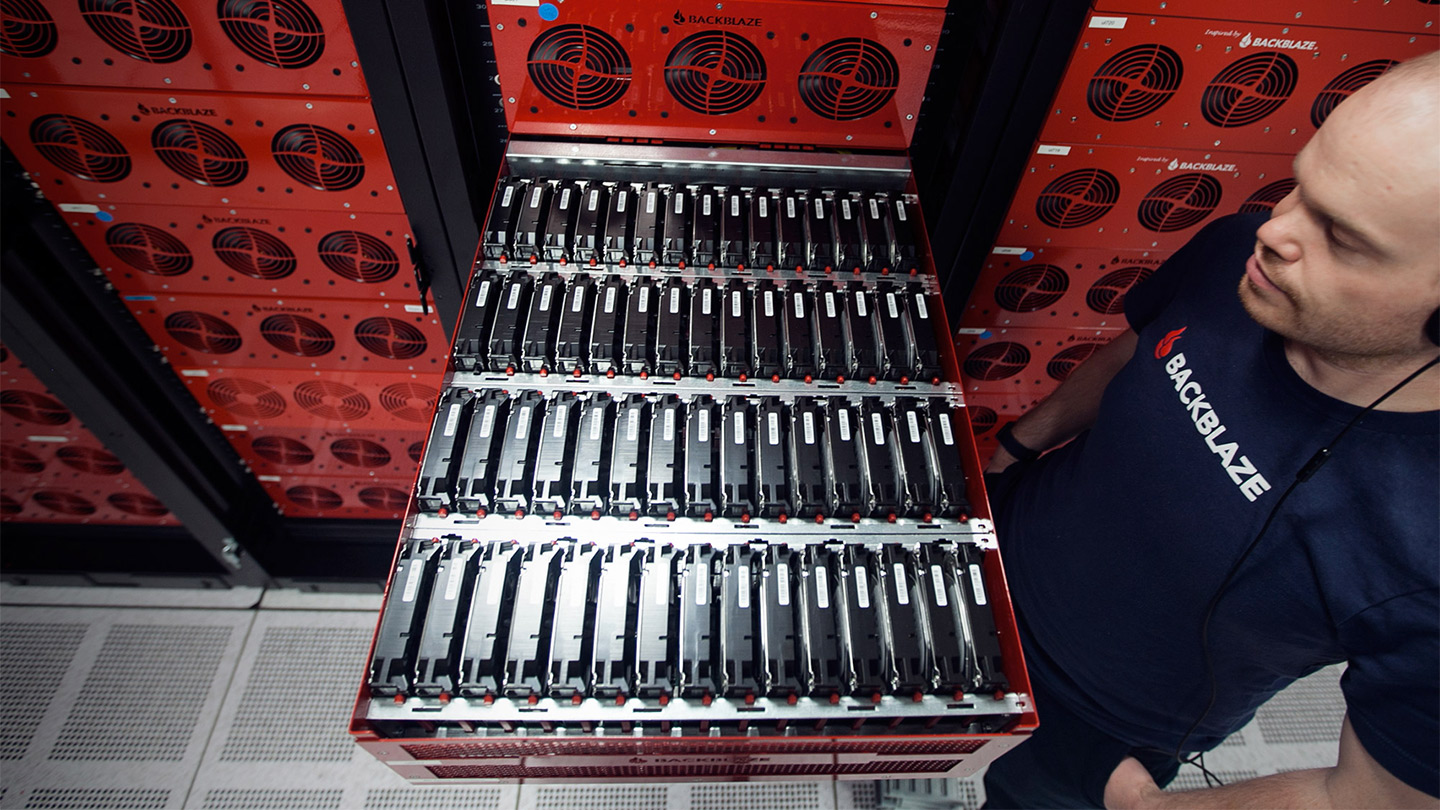
\includegraphics[scale=0.15]{../pictures/ZFS-Intro.png}
        \linebreak
        \only<2->{\textit{Workshop!}}
    \end{frame}

    \section{Was ist ZFS?}\label{sec:was-ist-zfs}
    \begin{frame}
        \slidehead
        \begin{itemize}[<+->]
        \item Zetta File System (ZFS) ist ein fortschrittliches Dateisystem, das ursprünglich von Sun Microsystems entwickelt wurde.
        \item Es ist in der Lage, mehrere Festplatten zu einem logischen Pool zu kombinieren und eine Vielzahl von Funktionen wie Datensicherheit, Effizienz, Verwaltung und Skalierbarkeit zu bieten.
        \item ZFS ist ein 128-Bit-Dateisystem, das eine maximale Kapazität von 256 Quadrillionen Zettabytes (ZB) bietet.
        \item ZFS kann in vielen Betriebssystemen verwendet werden - TrueNAS, FreeBSD, Linux, macOS, (windows)
        \end{itemize}
    \end{frame}

    \section{Bestandteile von ZFS}\label{sec:bestandteile-von-zfs}
    \begin{frame}
        \slidehead
        \begin{itemize}[<+->]

        \item Pool
        \begin{itemize}
            \item besteht aus einem oder mehreren Vdevs
            \item virtueller Pool, der auf mehrere physische Geräte aufgeteilt werden kann
        \end{itemize}

        \item Vdev (Virtual Device)
        \begin{itemize}
            \item besteht aus einer oder mehreren physischen Festplatten
            \item kann Spiegelung, RAID-Z, oder einzelne Festplatten enthalten
        \end{itemize}

        \item Dataset
        \begin{itemize}
            \item logische Gruppierung von Daten
            \item kann Eigenschaften wie Komprimierung, Verschlüsselung und Snapshots haben
        \end{itemize}

        \end{itemize}
    \end{frame}

    \section{Use-case}\label{sec:use-case}
    \begin{frame}[c]
        \begin{columns}[c]
            \begin{column}{.5\textwidth}
                \centering
                \includesvg{../pictures/bob}
            \end{column}
            \begin{column}{.5\textwidth}
                \Large
                \textcolor{TUDa-8a}{\textbf{Meet Bob}}
                \only<2->{
                    \begin{itemize}
                        \item<2-> Bob hat dateien, die er gerne behalten möchte
                        \item<3-> Bob möchte diese Dateien auf seinem Computer sicher speichern
                        \item<4-> Bob hat gehört, dass ZFS ein sicheres Dateisystem ist
                        \item<5-> Bob ist sich aber nicht sicher, was genau die Vorteile von ZFS sind
                    \end{itemize}
                }
            \end{column}
        \end{columns}
    \end{frame}

    \section{Vorteile von ZFS}\label{sec:vorteile-von-zfs}
    \begin{frame}
        \begin{columns}
            \begin{column}{.5\textwidth}
                \centering
                \Large
                \textcolor{TUDa-1b}{\textbf{ZFS}}
                \only<3->{
                    \begin{itemize}
                        \item Copy-On-Write (COW)
                        \item<4-> Checksumming
                        \item<5-> Native RAID-Z, Mirror, Stripe
                        \item<6-> Instant snapshots \& cloning
                    \end{itemize}
                }
            \end{column}
            \begin{column}{.5\textwidth}
                \only<2->{
                    \centering
                    \Large
                    \textcolor{TUDa-3b}{\textbf{ext4}}
                }
                \only<3->{
                    \begin{itemize}
                        \item Journaled
                        \item<4-> No file integrity checks
                        \item<5-> Single disk - limited scaling
                        \item<6-> No built-in snapshots/cloning
                    \end{itemize}
                }
            \end{column}
        \end{columns}
    \end{frame}

    \subsection{Copy on Write (COW)}\label{subsec:copy-on-write}
    \begin{frame}
        \slidehead
        \begin{itemize}[<+->]
            \item Daten werden nicht überschrieben, sondern immer in einem neuen Block geschrieben
            \item \url{https://arstechnica.com/information-technology/2020/05/zfs-101-understanding-zfs-storage-and-performance/3/}
        \end{itemize}
    \end{frame}

    \begin{frame}
        \slidehead
            \centering
            \vspace{-1.5em}
            \tiny
            \begin{table}[h]
                \renewcommand{\arraystretch}{.9}
                \begin{tabular}{lcccccc}
                    \toprule
                    & SEQ1MQ8T1 & SEQ128KQ8T1 & RND4KQ32T16 & RND4KQ1T1 \\
                    \midrule
                    Single no slog & 261 & 158 & 1008 & 618 \\
                    Single Slog & 270 & 250 & 1480 & 692 \\
                    16x stripe no slog & 323 & 155 & 12032 & 762 \\
                    16x stripe slog & 694 & 522 & 10470 & 1052 \\
                    8x mirror no slog & 287 & 130 & 8627 & 963 \\
                    8x mirror slog & 661 & 472 & 8627 & 892 \\
                    1x RAID-Z1 no slog & 341 & 76 & 2944 & 585 \\
                    1x RAID-Z1 slog & 705 & 502 & 15744 & 1901 \\
                    1x RAID-Z2 no slog & 341 & 75 & 2867 & 600 \\
                    1x RAID-Z2 slog & 698 & 508 & 13952 & 1967 \\
                    1x RAID-Z3 no slog & 342 & 75 & 2969 & 581 \\
                    1x RAID-Z3 slog & 742 & 499 & 15027 & 2007 \\
                    2x RAID-Z1 no slog & 396 & 94 & 3968 & 864 \\
                    2x RAID-Z1 slog & 697 & 513 & 14182 & 1575 \\
                    2x RAID-Z2 no slog & 384 & 94 & 3916 & 870 \\
                    2x RAID-Z2 slog & 648 & 494 & 13081 & 1610 \\
                    2x RAID-Z3 no slog & 366 & 92 & 3814 & 807 \\
                    2x RAID-Z3 slog & 668 & 481 & 11852 & 1567 \\
                    4x RAID-Z1 no slog & 377 & 123 & 6092 & 1153 \\
                    4x RAID-Z1 slog & 697 & 495 & 12262 & 1149 \\
                    4x RAID-Z2 no slog & 378 & 115 & 5555 & 1046 \\
                    4x RAID-Z2 slog & 643 & 470 & 10137 & 1086 \\
                    4x RAID-Z3 no slog & 315 & 98 & 4608 & 995 \\
                    4x RAID-Z3 slog & 529 & 407 & 5555 & 861 \\
                    \bottomrule
                \end{tabular}
                \caption{ZFS vs ext4 performance comparison}
                \label{tab:zfs_ext4_comparison}
            \end{table}
    \end{frame}
\end{document}
